\section{High level components and their interaction}
\label{sec:high-level}

The main high level components of the system are the following:
\begin{description}
	\item[Database:] the data layer is responsible for the data storage and retrieval. It does not implement any application logic. This layer must guarantee ACID properties.
	\item[Application server:] this layer contains all the application logic of the system. All the policies, the algorithms and the computation are performed here. This layer offers a service-oriented interface.
	\item[Server side plug-ins:] these are the plug-ins which can be used to extend the application server layer. In this document, two plugins will be designed:
		\begin{itemize}
		\item ride sharing
		\item ride reservation
		\end{itemize}
	\item[Web server:] this presentation layer provides a web interface. This layer does not contain any application logic.
	\item[Mobile application:] this presentation layer consists in the mobile client. It communicates directly with the application server.
	\item[User's browser:] this presentation layer represents the user's browser; it is not under the control of the system and it accesses the web server.
\end{description}

These high-level components are structured into four layers, shown in figure \ref{fig:layers}.

This design choice makes it possible to deploy the application server and the web server on different tiers. It also improves scalability, since there may be many web servers talking to a single application server. Further implementations may include the use of caching at the web server level.

\begin{figure}[h]
\centering
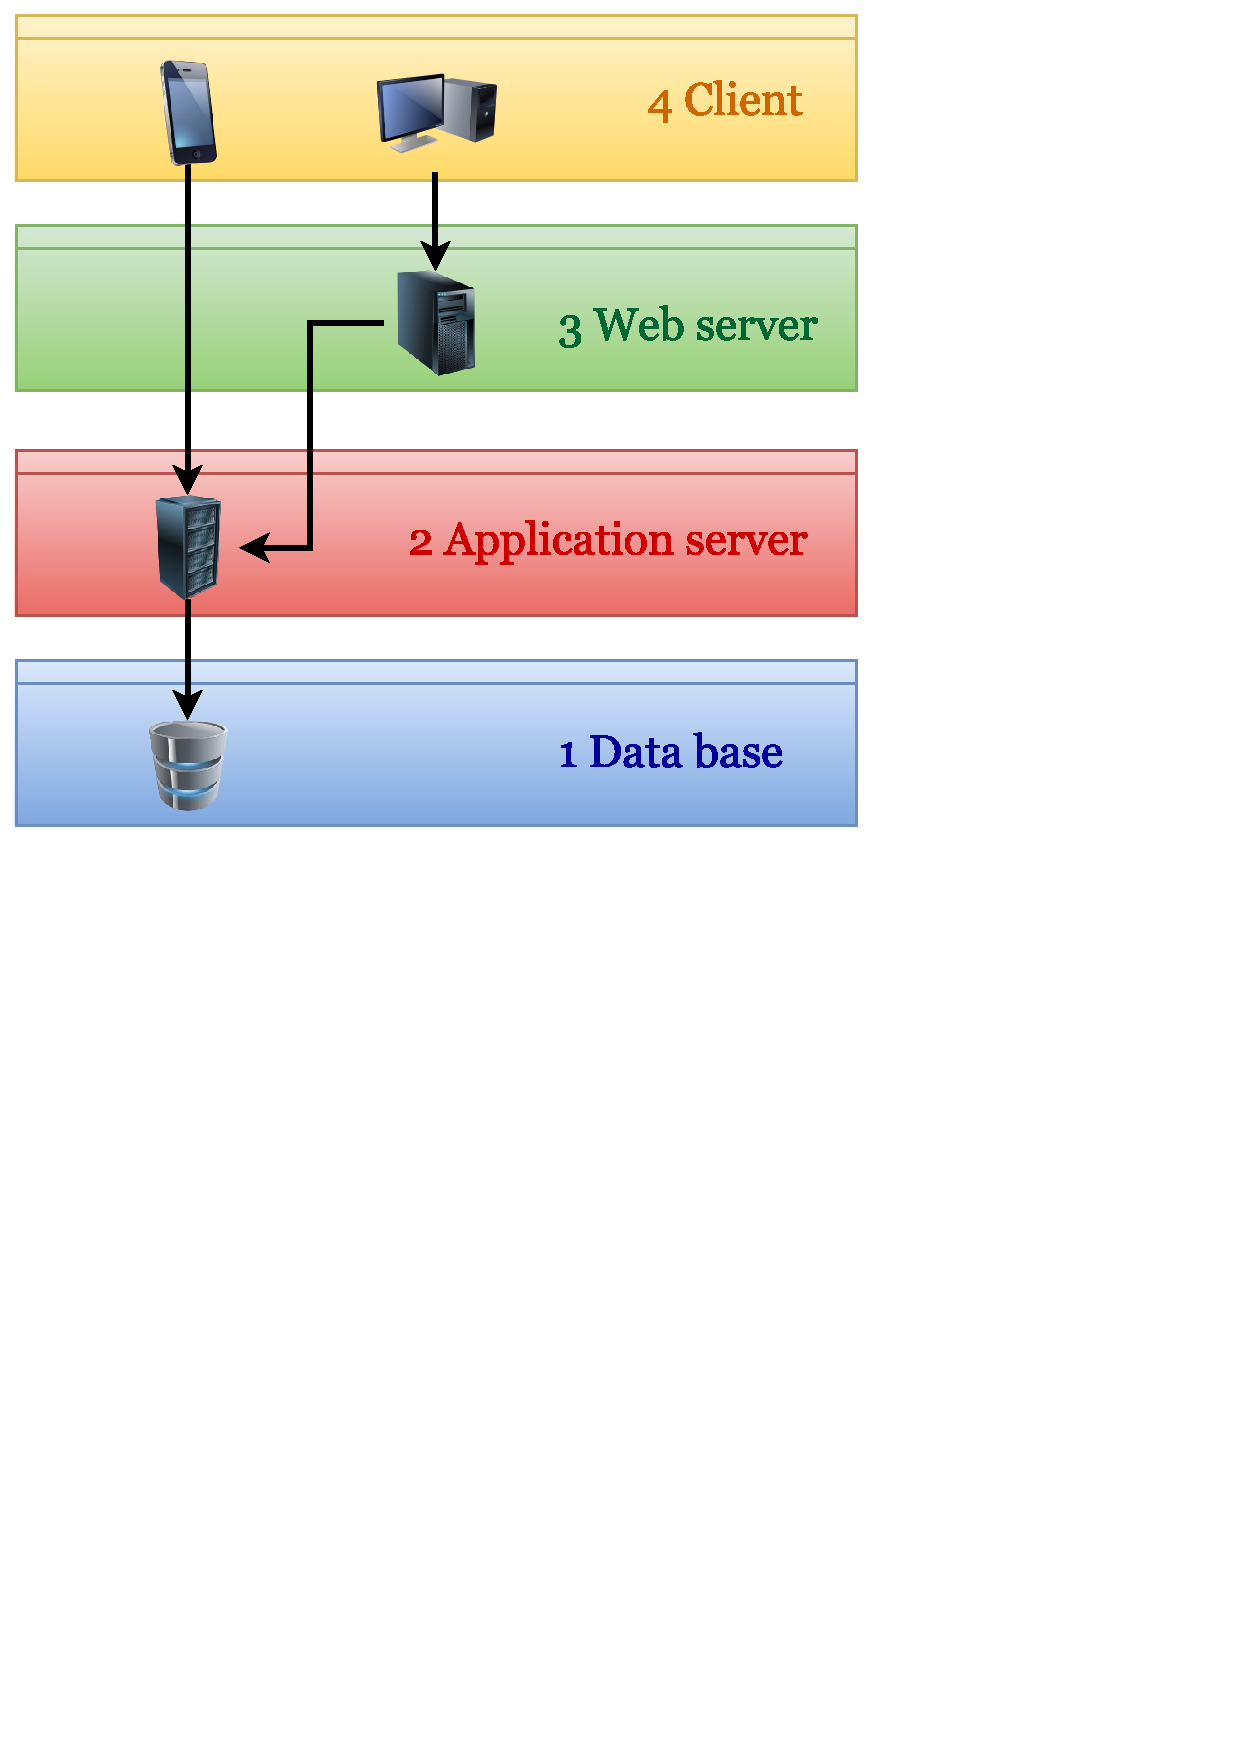
\includegraphics[width=0.7\textwidth]{diagrams/layers.pdf}
\caption{Layers of the system.}
\label{fig:layers}
\end{figure}

The interactions between the main components are shown in the figure \ref{fig:high_level_components}. They are all synchronous (obviously, the web server and the application server are multi-threaded).

\begin{figure}[h]
\centering
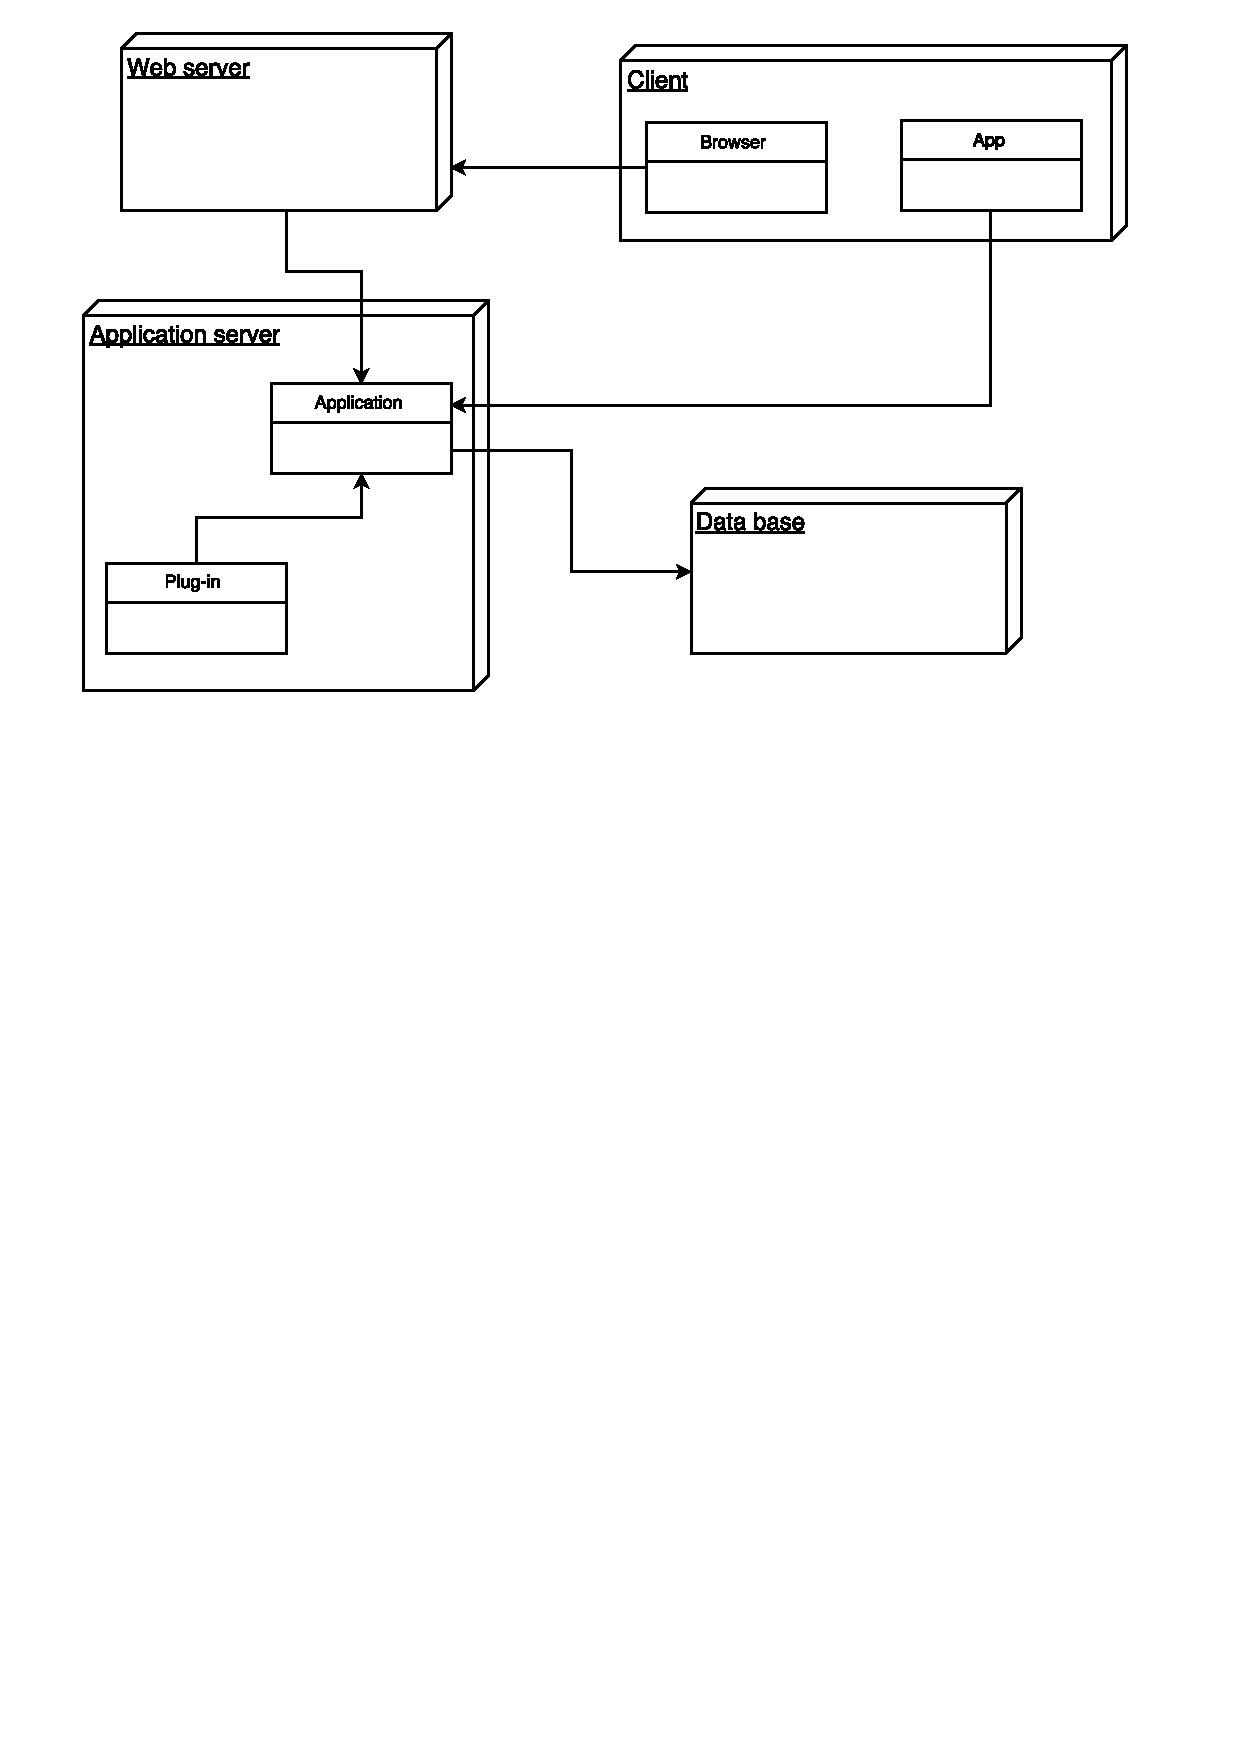
\includegraphics[width=\textwidth]{diagrams/high_level_components.pdf}
\caption{High level components of the system.}
\label{fig:high_level_components}
\end{figure}
